\documentclass[tikz,border=8pt]{standalone}
% Shared look for every TikZ diagram. Load with \input{../../tools/tikz-style.tex}
\usepackage[sfdefault]{roboto}
\usetikzlibrary{arrows.meta, positioning, shapes.geometric, calc, fit, backgrounds}
\definecolor{cblue}{HTML}{4C78A8}
\definecolor{corange}{HTML}{F58518}
\definecolor{cgreen}{HTML}{54A24B}
\definecolor{cred}{HTML}{E45756}
\definecolor{cpurple}{HTML}{B279A2}
\definecolor{cgrey}{HTML}{6B6B6B}
\tikzset{
  every picture/.style={font=\sffamily, line width=1.2pt},
  box/.style={draw=#1, fill=#1!12, rounded corners=4pt, align=center, inner sep=7pt, minimum height=1.1cm},
  box/.default=cgrey,
  arrow/.style={-{Stealth[length=3mm]}, draw=cgrey, line width=1.4pt},
  title/.style={font=\sffamily\bfseries\Large},
  note/.style={font=\sffamily\small, text=cgrey, align=center},
}
\AtBeginDocument{\hyphenpenalty=10000 \exhyphenpenalty=10000}

% Two subsumption levels for the room robot, after Brooks (1986), levels 0 and 1 (as described in Dean, CS148
% "Architectures"): level 0 = collide (halt) + feelforce (push) + runaway; level 1 = a goal behaviour whose avoid
% module combines its own steering with the push and suppresses runaway's output (S). Collide's halt is never
% suppressed. Ours: level 1 steers to the lamp with the Braitenberg 3a wiring.
\begin{document}
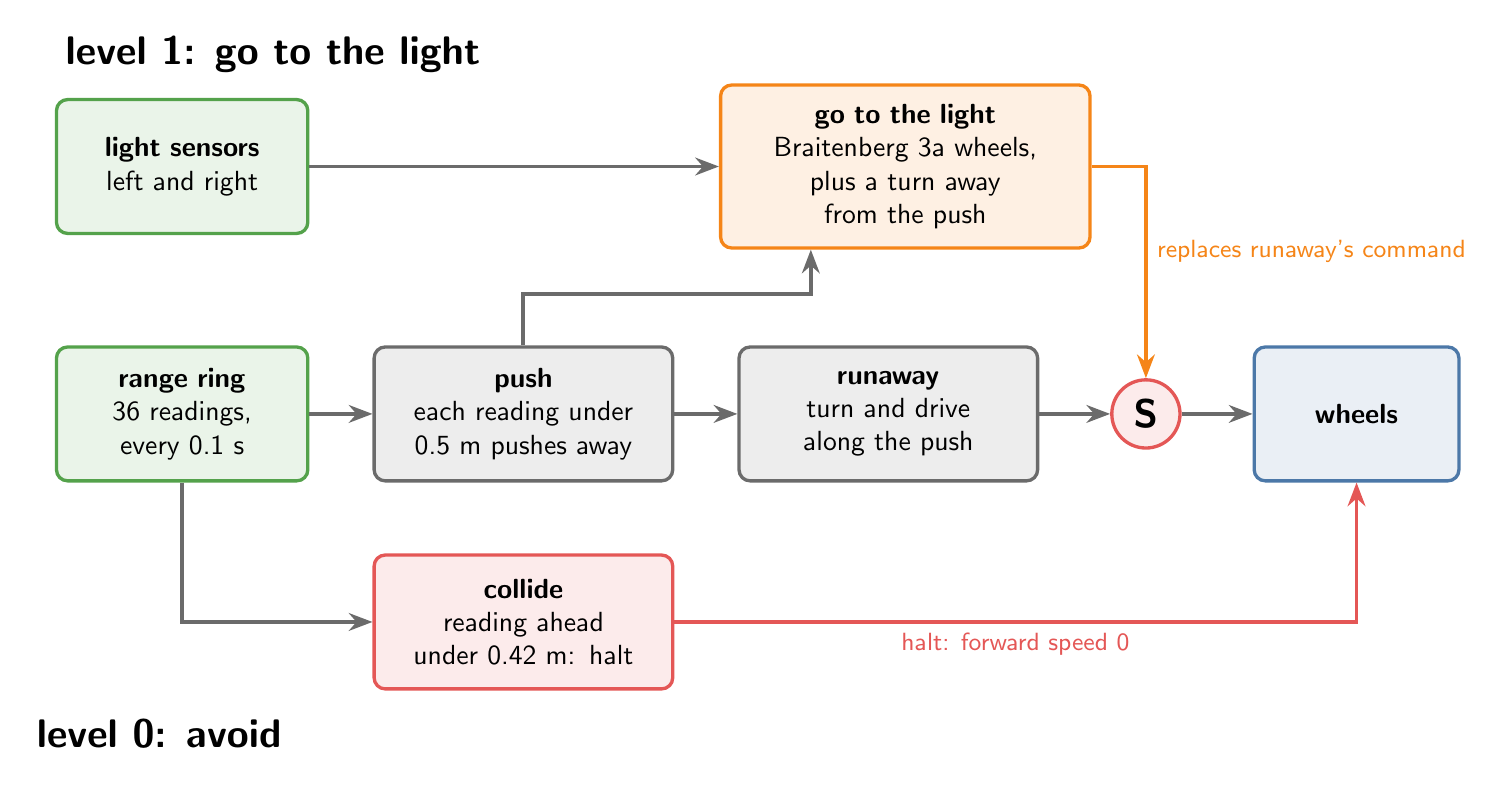
\begin{tikzpicture}[node distance=0.8cm,
  m/.style={box=#1, minimum width=3.6cm, text width=3.3cm, minimum height=1.7cm},
  sens/.style={box=cgreen, minimum width=3.0cm, text width=2.7cm, minimum height=1.7cm}]
  % level 0
  \node[sens] (ring) {\textbf{range ring}\\ 36 readings,\\ every 0.1 s};
  \node[m=cgrey, right=of ring] (push) {\textbf{push}\\ each reading under\\ 0.5 m pushes away};
  \node[m=cgrey, right=of push] (run) {\textbf{runaway}\\ turn and drive\\ along the push};
  \node[circle, draw=cred, fill=cred!12, font=\sffamily\bfseries\Large, inner sep=4pt, right=0.9cm of run] (S) {S};
  \node[box=cblue, minimum width=2.6cm, minimum height=1.7cm, right=0.9cm of S] (wh) {\textbf{wheels}};
  \node[m=cred, below=0.9cm of push] (col) {\textbf{collide}\\ reading ahead\\ under 0.42 m: halt};
  % level 1
  \node[sens, above=1.4cm of ring] (light) {\textbf{light sensors}\\ left and right};
  \node[m=corange, right=of light, xshift=4.4cm, text width=4.2cm, minimum width=4.5cm] (go) {\textbf{go to the light}\\ Braitenberg 3a wheels,\\ plus a turn away\\ from the push};
  \draw[arrow] (ring) -- (push);
  \draw[arrow] (push) -- (run);
  \draw[arrow] (run) -- (S);
  \draw[arrow] (S) -- (wh);
  \draw[arrow] (ring.south) |- (col.west);
  \draw[arrow, cred] (col.east) -| node[note, pos=0.25, below, text=cred] {halt: forward speed 0} (wh.south);
  \draw[arrow] (light) -- (go);
  \draw[arrow] (push.north) -- ++(0,0.65) -| ($(go.south)+(-1.2,0)$);
  \draw[arrow, corange] (go.east) -| node[note, pos=0.7, right, text=corange] {replaces runaway's command} (S.north);
  \node[title, anchor=west] at ($(light.north west)+(0,0.55)$) {level 1: go to the light};
  \node[title, anchor=west] at ($(col.south west)+(-4.4,-0.55)$) {level 0: avoid};
\end{tikzpicture}
\end{document}
